\newcommand\altfm[1][$\dagger$]{\textsuperscript{#1}}
\newcommand\altft[2][$\dagger$]{\footnotesize{\altfm[#1] #2}}
\newcommand\altfr{\vfill\rule{16em}{0.4pt}\par}
\newcommand\by[1]{\text{\footnotesize{(#1)}}}

\subsection{Siegel's Linearisation Theorem}
\begin{frame}{Siegel's Linearisation Theorem}
\begin{theorem}[Siegel 1942]
If $\xi$ is Diophantine of any order, then every germ of a holomorphic map with fixed point of multiplier $\lambda = e^{2\pi i\xi}$ is locally linearisable.
\end{theorem}\pause

\begin{theorem}[Quadratic Siegel discs exist]
For Lebesgue-almost all irrational $\lambda \in \R/\Z$, $f_\lambda(z) = \lambda z + z^2$ has a Siegel disc about the origin.
\end{theorem}

This is strictly weaker than Siegel (1942).
\end{frame}

\subsection{Siegel's Linearisation Theorem (Weak Version)}

\begin{frame}
\begin{thm}[Riemann mapping theorem]
Let $U \subset \C$ be a simply connected domain. Then for every $z_0 \in U$ there is a unique conformal isomorphism $\phi: U \to \D$ to the unit disc such that
\[
\phi(z_0) = 0 \quad\text{and}\quad \phi'(z_0) > 0
\]
\end{thm}
\pause
\begin{dfn}[Conformal radius] The \emph{conformal radius} of $U$ as viewed from $z_0 \in U$ is $\operatorname{rad}(U, z_0) = \dfrac{1}{\phi'(z_0)}$.
\end{dfn}
\pause
\emph{Intuition:} requiring instead $\phi: U \to \D_r$ with $\phi'(0) = 1$:
\[
\begin{tikzcd}[ampersand replacement=\&]
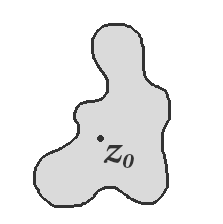
\includegraphics[width=0.2\textwidth]{resources/ch-11/uniformisation-blob.png}
\ar[r, "\phi",
start anchor={[yshift=.08\textwidth]},
end anchor={[yshift=.08\textwidth]}] \&

\includegraphics[width=0.2\textwidth]{resources/ch-11/uniformisation-circle.png}
\end{tikzcd}
\]
\end{frame}

\begin{frame}
    \begin{dfn}[Conformal radius function]
    For $\lambda \in \C$, let $\sigma(\lambda)$ be the conformal radius from $0$ of the maximal neighbourhood about $0$ on which $f_\lambda$ is conjugate to a rotation.
    
    \pause
    If no such neighbourhood exists, set $\sigma(\lambda) = 0$.
    \end{dfn}
    \pause

    Some properties:
    \begin{itemize}
        \item $\sigma$ is non-constant ($\sigma(0) = 0$, $\sigma(\lambda) > 0$ for $\abs{\lambda} \notin \{0, 1\}$.)
        \item $\sigma$ is \emph{upper semi-continuous} on $\cl{\D}$. 
    \end{itemize}
    
\end{frame}

\begin{frame}
\begin{itemize}
    \item When $\abs{\lambda} < 1$, Koenigs linearisation:
\end{itemize}

\[
\begin{tikzcd}[ampersand replacement=\&]
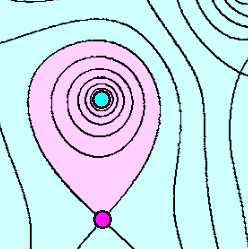
\includegraphics[width=0.2\textwidth]{resources/ch-11/julia-attracting-local.png}
\ar[r, "\phi",
start anchor={[yshift=.08\textwidth]},
end anchor={[yshift=.08\textwidth]}] \&
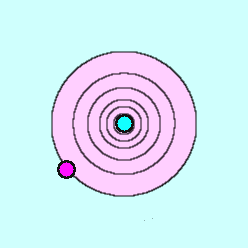
\includegraphics[width=0.2\textwidth]{resources/ch-11/julia-circle.png}
\end{tikzcd}
\]

\pause
\begin{itemize}
    \item $\eta(\lambda) = \phi({\color{magenta}-\lambda/2})$. The function $\eta(\lambda)$ is holomorphic on the punctured disc. The singularity at the origin is removable --- have $\sigma(\lambda) = \abs{\eta(\lambda)}$ on $\D$.
    \pause \item Computation:
    \[
\eta(\lambda) = -\frac{\lambda}{4} + \frac{\lambda^2}{16}
+\frac{\lambda^3}{16} + \frac{\lambda^4}{32} + \frac{9\lambda^5}{256} + \frac{\lambda^6}{256} +
\frac{7\lambda^7}{256} + O(\lambda^8)
\]
\end{itemize}

\end{frame}

\begin{frame}
\begin{lem}[F. and M. Riesz, 1916]\label{lem:A.3}
    Let $\eta: \D \to \C$ be bounded and holomorphic. If for some constant $c \in \C$ the set of $\xi$ such that
    \[
    \lim_{r\nearrow 1} \eta (r e^{2\pi i \xi}) = c
    \]
    has positive Lebesgue measure, then $\eta$ is constant.
\end{lem}
\vspace{1em}
\pause

\begin{proof}[Proof (quadratic Siegel discs exist)]

$\displaystyle \phantom{=}\ \{ \xi \in \R/\Z \mid
   z \mapsto e^{2\pi i \xi} z + z^2 \text{ not linearisable at $z = 0$} \}$

$\displaystyle = \{ \xi \in \R/\Z \mid
    \sigma(e^{2\pi i \xi}) = 0 \}$ \hfill {\footnotesize(by definition of $\sigma$)}

$\displaystyle = \{ \xi \in \R/\Z \mid
    \lim_{r \nearrow 1} \eta(r e^{2\pi i \xi}) = 0 \} $ \hfill {\footnotesize(upper semi-continuity)}
    
is a set of Lebesgue measure zero.
\end{proof}
\end{frame}

% Stronk version

\subsection{Siegel's Linearisation Theorem}
\begin{frame}{Siegel's Linearisation Theorem}
Strong version.

\begin{theorem}[Siegel 1942]
If $\xi$ is Diophantine of any order, then every germ of a holomorphic map with fixed point of multiplier $\lambda = e^{2\pi i\xi}$ is locally linearisable.
\end{theorem}
\end{frame}

\begin{frame}
\emph{Schröder's equation:} given $f$, seek $\psi$ such that $f(\psi(z)) = \psi(\lambda z)$
\[
\begin{tikzcd}[ampersand replacement=\&]
\C \ar[r, "f"] \& \C\\
\D_r \ar[u, "\psi"] \ar[r, "w \mapsto \lambda w"'] \& \D_r \ar[u, "\psi"']
\end{tikzcd}
\]
\pause
Up to first order:
\begin{itemize}
    \item $\psi(z) = z + \Psi(z)$
    \item $f(z) = \lambda z + F(z)$
\end{itemize}

Attempt instead to solve $F(z) = \Psi(\lambda z) - \lambda\Psi(z)$:
\pause
\[
    \Psi_0(z) = \sum_{j=2}^\infty \frac{b_j}{\lambda^j - \lambda}z^j
\]
in which $b_j$ are coefficients of the series expansion $F(z) = \sum_{j=2}^\infty b_j z^j$.
\end{frame}


% BRUTE FORCE BECAUSE
\begin{frame}
\[
\begin{tikzcd}[ampersand replacement=\&]
\D_{r_0} \ar[r, "f_0 = f"] \&[12em] \C
\ar[d, "\psi_0\inv"]
\\
\D_{r_1} \ar[u, "\psi_0"]
\ar[r, "f_1 = \psi_0 \circ \inv f \circ \psi_0"]
\&{}
\\
{}\&{} \\
{}\&{} \\
{}\&{}
\end{tikzcd}
\]
\end{frame}
\begin{frame}
\[
\begin{tikzcd}[ampersand replacement=\&]
\D_{r_0} \ar[r, "f_0 = f"] \&[12em] \C
\ar[d, "\psi_0\inv"]
\\
\D_{r_1} \ar[u, "\psi_0"]
\ar[r, "f_1 = \psi_0 \circ \inv f \circ \psi_0"]
\&
\ar[d, "\psi_1\inv"]
\\
\D_{r_2} \ar[u, "\psi_1"]
\ar[r, "f_2 = \psi_1\inv \circ \psi_0 \circ \inv f \circ \psi_0 \circ \psi_1"]
\&
\ar[d, "\psi_2\inv"] \\
\vdots
\ar[u, "\psi_2"]
\&
\vdots\\
{}
\&
{}
\end{tikzcd}
\]
\end{frame}

\begin{frame}
\[
\begin{tikzcd}[ampersand replacement=\&]
\D_{r_0} \ar[r, "f_0 = f"] \&[12em] \C
\ar[d, "\psi_0\inv"]
\\
\D_{r_1} \ar[u, "\psi_0"]
\ar[r, "f_1 = \psi_0 \circ \inv f \circ \psi_0"]
\&
\ar[d, "\psi_1\inv"]
\\
\D_{r_2} \ar[u, "\psi_1"]
\ar[r, "f_2 = \psi_1\inv \circ \psi_0 \circ \inv f \circ \psi_0 \circ \psi_1"]
\&
\ar[d, "\psi_2\inv"] \\
\vdots
\ar[r, color=white, "\textit{\color{black}(hopefully)}"']
\ar[u, "\psi_2"]
\&
\vdots\\
\D_{r_\infty} \ar[r, "z \mapsto \lambda z"]
\&
\D_{r_\infty}
\end{tikzcd}
\]
\end{frame}

\begin{frame}
Analysis ensues:
\begin{itemize}
    \pause \item Diophantine: $1/\abs{\lambda^q - 1} < M q^\kappa$
    \begin{itemize}
        \item $\abs{F_n}, \abs{\Psi_n} \tendsto 0$ fast enough
        \item $f_n$ tends to $z \mapsto \lambda z$; $\psi_n$ becomes close to the identity.
    \end{itemize}
    \pause \item Carefully check:
    \begin{itemize}
        \item Each $\psi_k, \psi_k\inv$ well-defined.
        \item $r_\infty > 0$.
    \end{itemize}
\end{itemize}
\end{frame}

\subsection{The Postcritical Closure}
\begin{frame}
What do Siegel discs \emph{look like?} \uncover<1->{Compare results from previous sections:}
\begin{minipage}{0.6\textwidth}
\begin{itemize}
    \item<1-> \emph{Attracting fixed point}:
    \begin{itemize}
        \item at least one critical point in {\color<1>{cyan}basin of attraction}.
        \item at least one critical point on boundary of
        {\color<1>{magenta} maximal linearising domain}.
    \end{itemize}
    %
    \item<2-> \emph{Parabolic fixed point} with $\lambda = 1$: 
    \begin{itemize}
        \item at least one critical point in each {\color<2>{cyan}immediate basin.}
        \item at least one critical point on boundary of {\color<2>{magenta}maximal attracting petal}.
    \end{itemize}
    %
    \item<3-> \emph{Irrationally indifferent fixed point}:
    \begin{itemize}
        \item are there critical points on the boundary of Siegel discs?
        \uncover<4->{
        \emph{Sometimes.\altfm}
    \vfill
    \altfr\altft{
    Herman M. 1985.
    \textit{Are there critical points on the boundaries of singular domains?}
    Comm. Math. Phys., 99(4):593–612}}
    \end{itemize}
\end{itemize}
\end{minipage}\hfill
\begin{minipage}{0.4\textwidth}
\includegraphics<1>[width=\textwidth]{resources/ch-11/julia-attracting.png}%
\includegraphics<2>[width=\textwidth]{resources/ch-11/julia-cauliflower.png}%
\includegraphics<3->[width=\textwidth]{resources/ch-11/julia-cauliflower-gs.png}%
\end{minipage}

\end{frame}
\begin{frame}
    \begin{dfn} The \emph{postcritical closure} of $f$ is the topological closure of the forward orbit of the set of critical points:
    \[
    P(f) = \cl{\bigcup_{k > 0} \iter{f}{k}(V(f))}
    \]
    where
    \[
    V(f) = \{ z \in \hat{\C} \mid f'(z) = 0 \}
    \]
    \end{dfn}
    \pause
    \par\vspace{1em}
    Equivalently, $P(f)$ is the smallest forward-invariant closed set containing all critical values of $f$.
\end{frame}

\subsection{The Postcritical Closure}
\begin{frame}
\begin{thm}
Each of the following sets is contained within $P(f)$:
\begin{itemize}
    \pause\item all (super-)attracting periodic orbits of $f$.
    \pause\item all indifferent periodic orbits which lie within $\julia(f)$.
    \pause\item the boundary of every period of rotation domains.
\end{itemize}
\end{thm}
\pause
\begin{proof}[Sketch of proof]
If $\abs{P(f)} < 3$: special case. $f$ is conjugate to $z \mapsto z^{\pm d}$.

Assume $\abs{P(f)} \ge 3$. Equip $Q = \hat{\C}\setminus P(f)$ with the \emph{Poincaré metric;} apply the Schwarz-Pick lemma to show that $\iter{f}{k}$ expands distances on $Q$.
\end{proof}
\end{frame}


\newcommand\imageonlyframe[3][1.0]{
{\setbeamercolor{background canvas}{bg=black}
\setbeamercolor{caption name}{fg=white}
\setbeamercolor{normal text}{fg=white}
\begin{frame}
\vfill
\begin{figure}
\includegraphics[width=#1\textwidth]{#2}
\caption{#3}
\end{figure}
\end{frame}
}}

\imageonlyframe[0.7]{resources/ch-11/siegel-example-a.png}{
Filled Julia set (grey) for $\xi \approx 0283$ with forward orbit of critical point (white) together with several other points (magenta, yellow, cyan). Critical orbit delineates rotation domain.}
\imageonlyframe{resources/ch-11/parabolic-and-siegel.png}{
A rotation domain in $\xi \approx 0.2949$ (right), and an attracting cycle of period 4 in $\xi = 0.25$ (left).
}
\imageonlyframe[0.7]{resources/ch-11/siegel-example-b.png}{
$\xi \approx 0.4892$. A rotation domain being `squeezed'.
} 
\imageonlyframe{resources/ch-11/siegel-sequence-2.png}{
Left to right: $\xi \approx 0.1543, 0.2475, 0.3408$. Shape of rotation domain suggestive of nearby rational numbers: $2/13, 1/4, 1/3$.
}

\section{References}
\begin{frame}{References}
\footnotesize

\begin{itemize}
\item Beardon, Alan F. 2000. \textit{Iteration Of Rational Functions}. New York, NY: Springer.

\item
Brjuno, Alexander D. 1965. \textit{Convergence of transformations of differential equations to normal forms}. Dokl. Akad. Nauk USSR 165, 987-989
(Soviet Math. Dokl., 1536-1538).

\item
Carleson, Lennart and Gamelin, Theodore W. 2013. \textit{Complex Dynamics}. New York, NY: Springer.

\item
Geyer, Lukas. 2016. \textit{Topics In Mathematics Complex Dynamics}. Lecture Notes, 2016.

\item
McMullen, Curtis T. 1994. \textit{Complex Dynamics and Renormalization.} Available from: \texttt{http://people.math.harvard.edu/~ctm/papers/home/text/papers/real/book.pdf}. Accessed June 2020.

\item
Milnor, John W. 2006. \textit{Dynamics In One Complex Variable}. Princeton, N.J.: Princeton University Press.

\item
Siegel, Carl L. 1942. \textit{Iteration of analytic functions}, Ann. of Math. (2) 43, 607–612. MR 7044

\item
Stoll, Danny. 2020. \textit{A Brief Introduction To Complex Dynamics}. University of Chicago. Accessed June 2020.
\end{itemize}
\end{frame}
